% !TEX program=lualatex

% nobabel means you'll need to provide your own month names, week day headings,
% etc
\documentclass[12pt,nobabel,sundayweek]{cdcalendar}

%% and here we do some settings for a calendar in Chinese
%% (*not* the lunar calendar! Just localising the Gregorian calendar into
%% Chinese)
\usepackage{zh-mod}

\setmainfont[Ligatures=TeX]{EB Garamond}
\setsansfont[Ligatures=TeX,BoldItalicFont=Fira Sans Italic,BoldFont=Fira Sans,Numbers=OldStyle]{Fira Sans Light}


\usepackage{graphicx}
\usepackage{fontawesome}
\usepackage{wallpaper}

\graphicspath{{img/}}

%% Define all event mark styles here
\tikzset{holiday/.style={rectangle,fill=orange!70}}
\tikzset{pink icon/.style={text=Pink,font=\large}}
\tikzset{blue icon/.style={text=SkyBlue,font=\large}}

\begin{document}

%%%%%%
% Cover
%%%%%%

% Remove this line if you feel the background pattern is too annoying
% \TileWallPaper{.5\paperwidth}{.5\paperheight}{ricepaper_v3}
\TileWallPaper{.5\paperwidth}{.1\paperheight}{lightpaperfibers}

% \coverBgColor{RoyalBlue!40!black}
\coverImage[(元)景德镇窑蓝釉白龙戏珠纹盘。BabelStone摄,CC BY-SA 3.0. \url{ https://commons.wikimedia.org/w/index.php?curid=19011812}]
{Yuan_Jingdezhen_dragon_and_pearl_dish}

\coverTitle[
font=\fontsize{30pt}{32pt}\kaishu\bfseries,
text width=\linewidth,align=flush right,red!50!RedViolet]
{二〇一七年历}

\makeCover
% 由于须要以LuaLaTeX编译,封面变换了字体大小以后,会影响到后面英汉字符之间的距离,只好再强行加这一行来修正。
\ltjsetparameter{xkanjiskip=.25\zw plus 1pt minus 1pt}

%%%% Remove this page if you don't need it --
%%%% just to show the actual output
{\centering
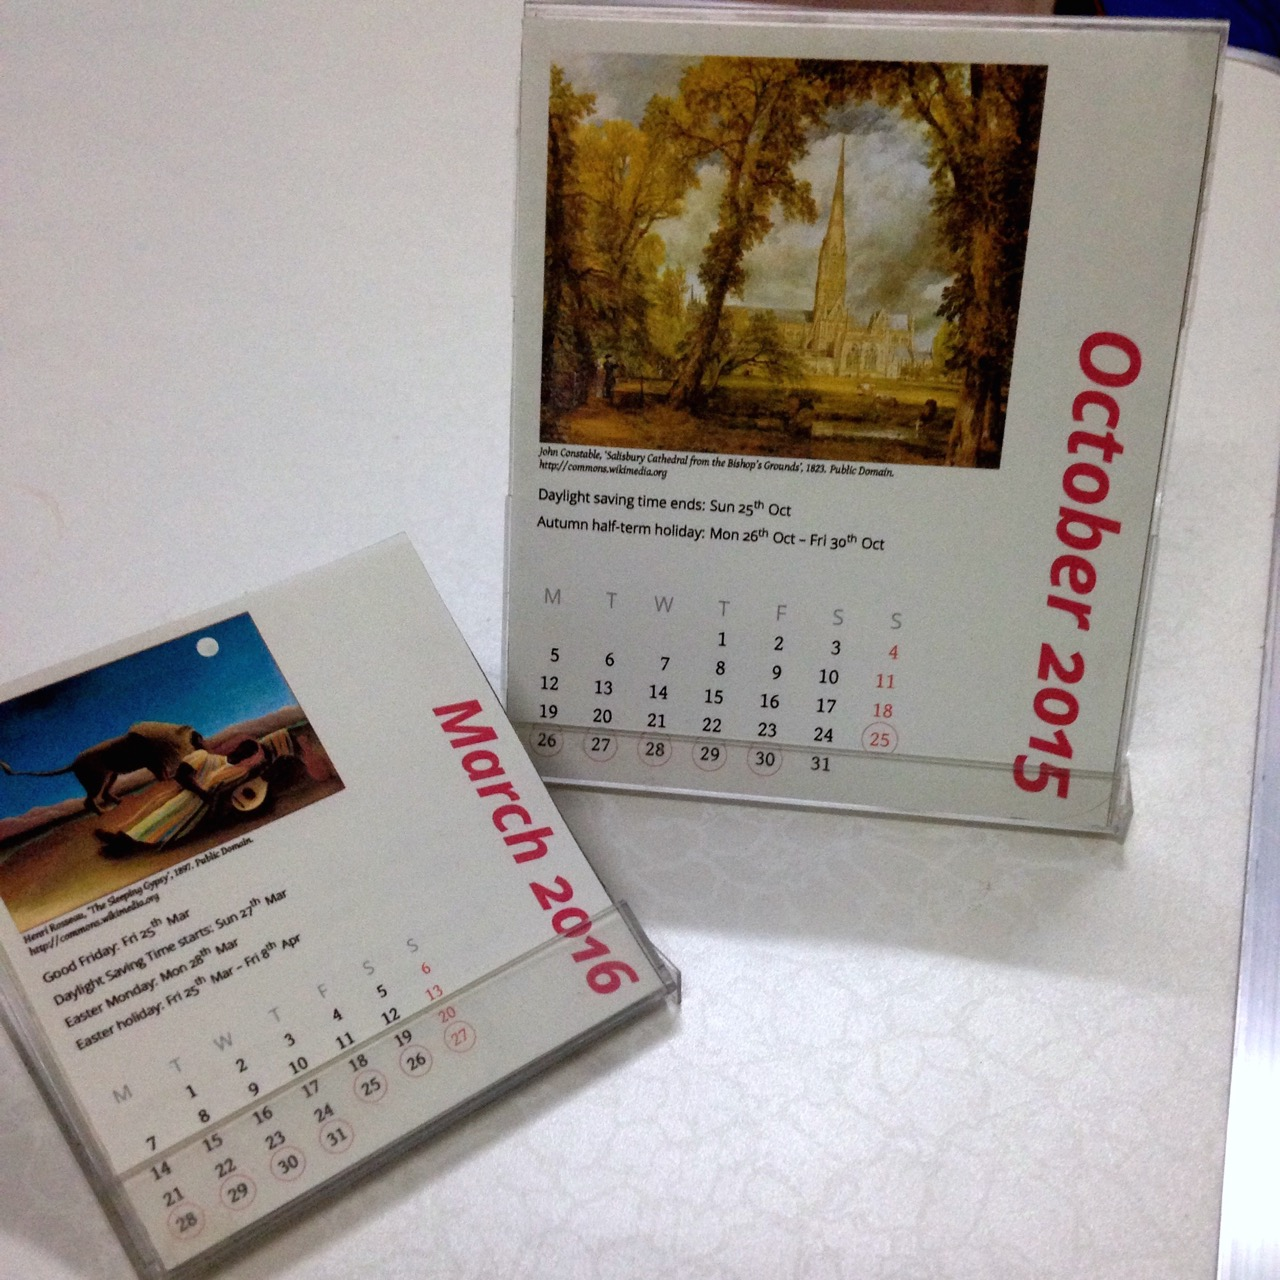
\includegraphics[width=\textwidth]{actual}
\par}

{\scriptsize
实际印刷出来的台历效果。较小尺寸的(\texttt{small} 选项,9\,cm $\times$ 9.5\,cm)适用3.5寸软盘盒(家里有这些古董的可以派上用场了)。较大尺寸的(默认设定,11.7\,cm $\times$ 13.65\,cm)则适用CD盒。另外还有\texttt{giant}选项,一页A4纸就一个月历。
\par}

\clearpage
%%%%

% You may find the gap between illustrations and events too wide
% Use this length to lessen it
\setlength{\lessIllusSkip}{1.5\ccwd}


%%%%%%
% Some settings for the monthly calendars
%%%%%%
\dayHeadingStyle{font=\sffamily\color{gray!90}}
\sundayColor{red}
\monthTitleStyle{font={\fontsize{42pt}{44pt}\bfseries\sffamily\fangsong}, red!50!RedViolet}
\eventStyle{\scriptsize\sffamily}

\illustration[花。金农, 1754。 公有领域(Public Domain). \url{http://bit.ly/2hed962}]
{8.5cm}{Flower_JinNong}


\begin{monthCalendar}{2017}{01}

\event[mark style=holiday]{2017-01-01}{2}{元旦+补休}
\event[mark style=holiday]{2017-01-27}{2017-2-2}{春节连休}
\event[mark style=blue icon, marker=\faBriefcase]
{2017-01-22}{}{春节调休上班}

\end{monthCalendar}

\clearpage

% 这一页"图"和月历距离可以大一些
\setlength{\lessIllusSkip}{0pt}
\otherstuff[金玉良言,苦口良药]
{8.5cm}{{\fontsize{48pt}{52pt}\fangsong\textcolor{red}{写}}%
        {\LARGE\kaishu,不停地写。}}

\begin{monthCalendar}{2017}{02}

\event[mark style=holiday]{2017-01-27}{2017-2-2}{春节连休}
\event[mark style=blue icon, marker=\faBriefcase]
{2017-02-04}{}{春节调休上班}
\event[mark style=pink icon,marker=\faBirthdayCake]{2017-02-14}{}{朋友生日}
\event{2017-02-22}{}{稿件死线!!}

\end{monthCalendar}

\end{document}
